\documentclass[main]{subfiles}

\begin{document}
\newpage
\thispagestyle{empty}
\begin{center}
    \centering
    
\includegraphics[width=0.25\linewidth]{LogoEjemplo.png} \par
    \vspace{3 cm}
    {\scshape\Huge Planos \par}
    \vspace{1.5cm}
    {\itshape\Huge \TituloProyecto \par}
    \vfill
    {\Large Solicitante:  \Solicitante \par}
    \vspace{0.5cm}
    {\Large Autor:  \Autor \par}
    \vspace{1.5cm}
    {\Large \Fecha \par}
\end{center}

% El documento que contiene los planos se iniciará con un índice que hará referencia a cada uno de ellos, indicando su ubicación, con el fin de facilitar su utilización.
\chapter*{Índice de planos:}
\tableof{Planos}
\toftagstart{Planos}
% Contendrán la información gráfica, alfanumérica, de códigos y de escala, necesaria para su comprensión.

% --------------------------- EJEMPLO ADJUNTAR PLANO -----------------------------------------
%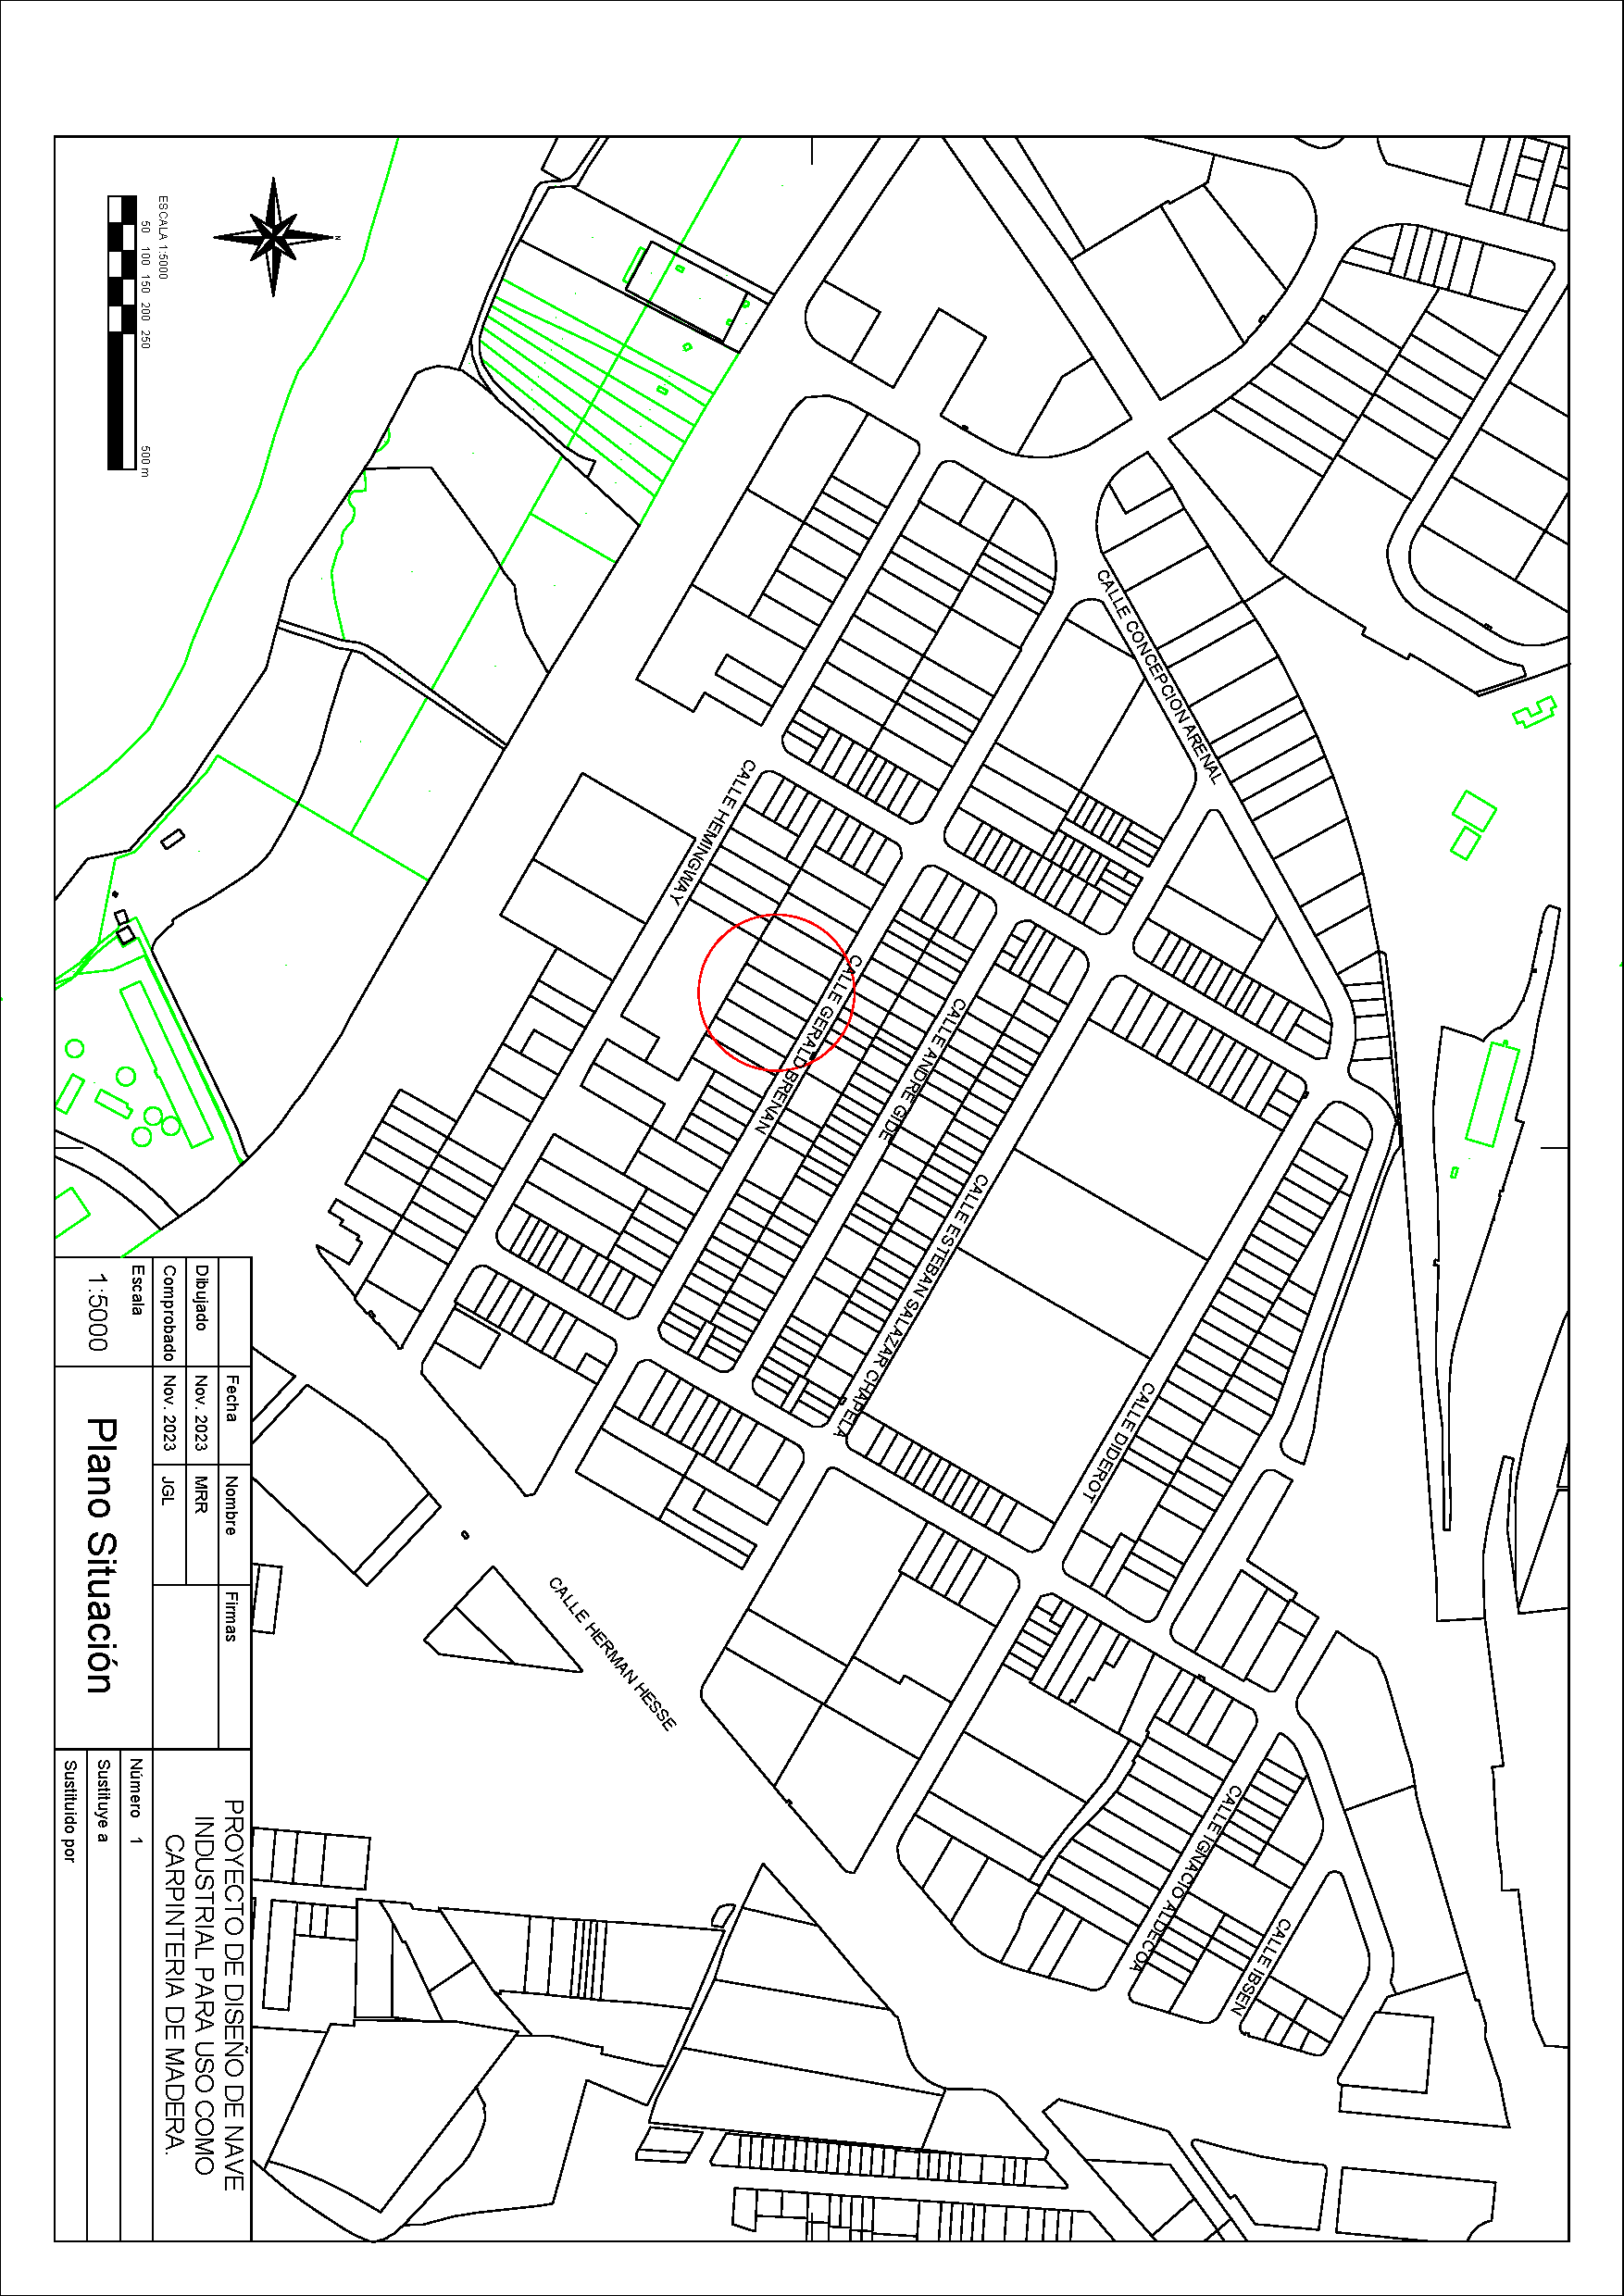
\includepdf[pages={1},pagecommand={
%    \thispagestyle{empty}
%    \addcontentsline{toc}{section}{Plano 1: Plano Situación}}]{Planos/Plano Situacion.pdf}
% --------------------------------------------------------------------------------------------

\toftagstop{Planos}
\end{document}